
\subsubsection{Multifont Strings}
%              -----------------
\label{sec:multifont}
%%%%%%%%%%%%%%%%%%%%%%%%%%%%%%%%%%%%%%%%%%%%%%%%%%%%%%%%%%%%%%%%%%%%%%%%%%%%%
%%%                             Description                               %%%
%%%%%%%%%%%%%%%%%%%%%%%%%%%%%%%%%%%%%%%%%%%%%%%%%%%%%%%%%%%%%%%%%%%%%%%%%%%%%
Any string can be displayed with multiple fonts referenced by font name aliases.
%%Font names are defined in a X11 resource file named Intens (see specification
%%example in section \nameref{sec:x-resources} page \pageref{sec:x-resources}).
\index{multifont strings}
\index{fonts}
\index{String!multifont strings}


%%\begin{boxedminipage}[t]{\linewidth}
%%\begin{verbatim}
%%Intens.*.fontList:
%%   -*-helvetica-*-r-*-*-12-*,\
%%   -*-clean-medium-r-*-*-14-*-*-*-*-*-iso8859-*=textfont,\
%%   -*-helvetica-bold-r-normal-*-14-*=hugefont,\
%%   -*-helvetica-bold-r-normal-*-12-*=largefont,\
%%   -*-helvetica-medium-r-normal-*-12-*=titlefont,\
%%   -*-helvetica-bold-r-normal-*-12-*=tabfont,\
%%   -*-helvetica-medium-r-normal-*-12-*=labelfont,\
%%   -*-helvetica-bold-r-*-*-12-*=indexfont,\
%%   -*-helvetica-bold-r-normal-*-12-*=menufont,\
%%   -*-helvetica-bold-r-normal-*-12-*=buttonfont,\
%%   -*-helvetica-medium-r-normal-*-12-*=pulldownfont,\
%%   -*-helvetica-medium-r-normal-*-14-*=bannerfont,\
%%   -*-helvetica-bold-r-normal-*-12-*=Title,\
%%   -*-symbol-medium-r-normal-*-12*-*=symfont
%%\end{verbatim}
%%\end{boxedminipage}


\index{  @Signs / Characters!\texttt{"@} (at)!multifont fontname delimiter}

%%A string composed of multiple fonts can now be created using fontnames specified
%%in resourcefiles like the example above. \\
Font names must be surrounded by two \verb+@+ characters. See example on page \pageref{sec:multifontexamples}. \\
The special fontname P switches back to the previously used font.\\

\input{diagrams/multifont_string}

\begin{tabularx}{\textwidth}{l|X}
Options    & Description \\
\hline
character  & any charachter sign except some described in section strings \nameref{sec:string} \\
P          & switches back to previous font \index{multifont strings!P}\\
fontname   & name of a font \\ %%must correspond to a previously declared alias in the \INTENS{} X11 resource file \\
\end{tabularx}

%%%%%%%%%%%%%%%%%%%%%%%%%%%%%%%%%%%%%%%%%%%%%%%%%%%%%%%%%%%%%%%%%%%%%%%%%%%%%
%%%                              Examples                                 %%%
%%%%%%%%%%%%%%%%%%%%%%%%%%%%%%%%%%%%%%%%%%%%%%%%%%%%%%%%%%%%%%%%%%%%%%%%%%%%%
%%\subsubsection{Examples}
\newpage
\label{sec:multifontexamples}

Example:


\begin{boxedminipage}[t]{\linewidth}
\begin{verbatim}
DESCRIPTION "Multifont strings";
UI_MANAGER
  FIELDGROUP
    fieldgroup_identifier (
      "@text@This is an example of a multifont string",
      "@text@========================================",
      "@text@text @huge@huge @large@large",
      "@titel@titel @tab@tab @label@label",
      "@index@index @menu@menu @button@button",
      "@pulldown@pulldown @banner@banner @Title@Title"
    );
  FORM
    form_identifier {MAIN} ((fieldgroup_identifier));
END UI_MANAGER;
END.
\end{verbatim}
\end{boxedminipage}

\vspace{0.5cm}

\begin{figure}[h]\label{fig:multifontString}
  \begin{center}
    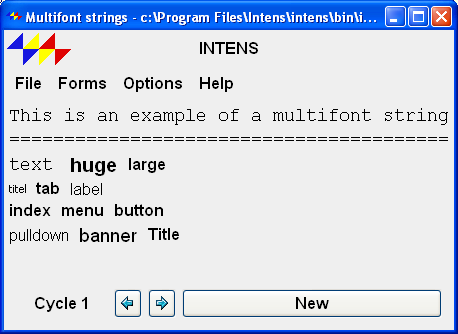
\includegraphics[width=0.5\linewidth]{grab_multifont}
  \end{center}
  \caption{Multifont string}
\end{figure}
